This example simulates the analytic solution derived by \cite{trahair2005nonlinear}.

A shaft is subjected to a concentrated torque $\TwistRxn$ acting at $\reflenx=L$. Rotation is prevented at the left support, $\reflenx=0$. 
The differential equation for nonlinear elastic nonuniform torsion is
%
\begin{equation}
G \Jsv \vartheta' - E \Jw \vartheta''' + \tfrac{1}{2} E I_n\left(\vartheta'\right)^3 = \TwistRxn
\tag{$\dagger$}
\end{equation}
%
where $\TwistRxn=$ torque at a distance $\reflenx$ along the torsion member; $\Jsv$ is the (Saint-Venant) uniform torsion section constant (\eqref{eq:def-j-origin}, $\Jw$ warping section constant; and $I_n$ is the  nonlinear ``Wagner'' section constant. 

The resultant torque $T$ comprises the linear uniform torque $G\Jsv \vartheta'$, the linear warping torque $-E\Jw \vartheta'''$, and the nonlinear torque $\tfrac12 E I_n \vartheta'''$ arising from the Wagner strain term \eqref{eq:wagner-gl-strain-pi}. 

\subsubsection{Uniform Twist}
\begin{figure}[H]
    \centering
    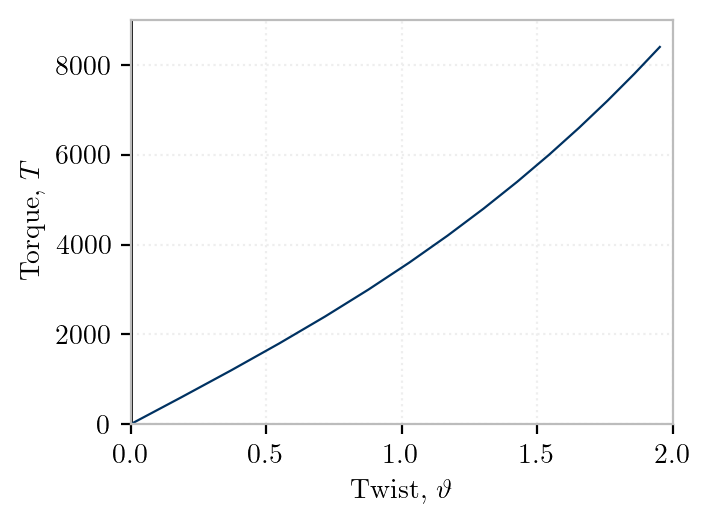
\includegraphics[width=0.5\linewidth]{Examples/frame-0015/img/e0010.png}
    \caption{Tip torque (\(\TwistRxn\)) vs. rotation (\(\vartheta\)) for Example~\ref{sec:frame-0015}.}
\end{figure}
This beam is in uniform torsion under a constant torque $\TwistRxn=M$, so that the twist $\vartheta'$ is constant along the member. 
In this case, ($\dagger$) can be solved in closed form as
$$
M=G J \frac{\vartheta_L}{L}+\tfrac{1}{2} E I_n\left(\frac{\vartheta_L}{L}\right)^3
$$
The section dimensions are $200 \mathrm{~mm} \times 10 \mathrm{~mm}$ with constants $J=66.667 \times 10^3 \mathrm{~mm}^4$, 
$\Jw=0 \mathrm{~mm}^6$, $I_n=17.778 \times 10^9 \mathrm{~mm}^6$, and length $L=1,000 \mathrm{~mm}$. 
% \begin{table}
\FrameSection{
label/problem=frame-0015,
%
shape=Rectangle,
kinematics/section={\eqref{eq:wagner-gl-strain-pi}},
% Cw=0,
J=66.667e3,
unit/length={\milli\meter},
% Material
E={200,000},
G={80,000},
unit/stress={\mega\pascal}
}
% \end{table}
This example has been considered by 
\cite{hsiao2000corotational,battini2002corotational,jonker2021threedimensional} \cite{rong2020geometrically} \cite{zhang2011formulation}.
